\documentclass{article}
\usepackage{tikz}
\usepackage{CJKutf8}
\usepackage{amsmath}
\usepackage{amsthm}
\begin{document}
\begin{CJK}{UTF8}{gbsn}
  \newtheorem*{Exercise}{习题}
  \huge
\begin{Exercise}[282-6]
  图$G$的最短圈的长度称为$G$的围长;如果$G$中没有圈,则定义$G$的围长为无穷大。
  证明:

  (i)围长为$r$的平面连通图$G$中有
  \[q \leq \frac{r(p-2)}{r-2}, r\geq 3\]

  (ii)利用(i)证明Petersen图不是可平面图。

  \centering
      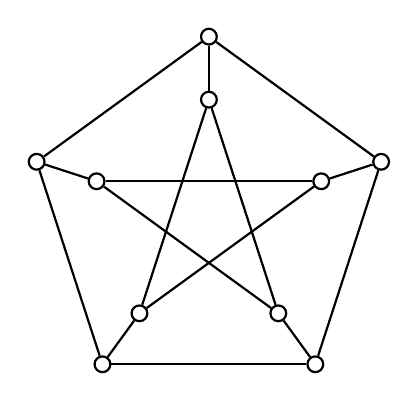
\begin{tikzpicture}[auto,
    specification/.style ={circle, draw, thick, inner sep = 0pt, minimum size=2mm}]
   \node[specification] (A)  at (18:2.3cm)  {};
   \node[specification] (B)  at (90:2.3cm)  {};
   \node[specification] (C)  at (162:2.3cm)  {};
   \node[specification] (D) at (234:2.3cm)  {};
   \node[specification] (E)  at (306:2.3cm)  {};
   \node[specification] (F)  at (18:1.5cm)  {};
   \node[specification] (G)  at (90:1.5cm)  {};
   \node[specification] (H)  at (162:1.5cm)  {};
   \node[specification] (I) at (234:1.5cm)  {};
   \node[specification] (J)  at (306:1.5cm)  {};
   
   
   \draw[thick] (A) to  (B);
   \draw[thick] (B) to  (C);
   \draw[thick] (C) to  (D);
   \draw[thick] (D) to  (E);
   \draw[thick] (E) to  (A);
   \draw[thick] (A) to  (F);
   \draw[thick] (B) to  (G);
   \draw[thick] (C) to  (H);
   \draw[thick] (D) to  (I);
   \draw[thick] (E) to  (J);
   \draw[thick] (G) to  (I);
   \draw[thick] (I) to  (F);
   \draw[thick] (F) to  (H);
   \draw[thick] (H) to  (J);
   \draw[thick] (J) to  (G);

 \end{tikzpicture}\\
 Petersen图  
\end{Exercise}

\end{CJK}
\end{document}


%%% Local Variables:
%%% mode: latex
%%% TeX-master: t
%%% End:
